% ====================================================================
%+
% SECTION:
%    WFIRST_microlensing.tex
%
% CHAPTER:
%    wfirst.tex
%
% ELEVATOR PITCH:
%
%
% AUTHORS:
%    David Bennett(@davidpbennett)
%-
% ====================================================================

\section{Exoplanetary Microlensing with WFIRST and LSST}
\def\secname{\chpname:microlensing}\label{sec:\secname}

\credit{davidpbennett},
\credit{mtpenny},
\credit{poleski},
{\it Rachel Street}.


Perhaps the most exciting discovery to come out of gravitational
microlensing surveys is the discovery of a large population of ``rogue"
planets by the MOA Collaboration \citep{2011Natur.473..349S}. These planets
are isolated in the sense that no host star can be detected
by microlensing. Depending on the peak magnification and light curve
coverage, this can imply that a host must be $> 10\,$AU or $> 100\,$AU away,
and \citet{2012ApJ...757..119B} have argued that the median separation
of possible host stars is likely to be $> 30\,$AU.
Further observations by both the MOA and OGLE collaborations provide
a qualitative confirmation of this result, as dozens of additional
short timescale events have been discovered by the MOA and OGLE
alert systems, but full details of the implied rogue planet
populations  will only come from detailed analyses of both the MOA
and OGLE samples.

A major weakness with the microlensing data that indicates this
large population of rogue planets is that, thus far, the properties
of this population have only been inferred by their Einstein radius
crossing time, $t_{\rm E}$, distribution. But, the Einstein radius crossing
time depends not only on the lens mass, but also on its distance and
transverse velocity. As a result, we cannot directly infer the mass or distance
distribution of the rogue planet sample.

Our understanding of the rogue planet distribution can be greatly improved
by measuring the microlensing parallax effect \citep{1992ApJ...392..442G,1995ApJ...454L.125A}.
The microlensing parallax effect can be described
by the transverse relative lens-source velocity, ${\bf v}_{\rm \perp}$, projected
to the position of the observer,
\begin{equation}
\tilde{\bf v} = {\bf v}_{\rm \perp} D_S/(D_S-D_L) \ , \label{eq-vp}
\end{equation}
where $D_L$ and $D_S$ are the lens and source distances, respectively.
Typically, microlensing parallax
is measured using the orbital motion of the Earth, but it can also be
measured using light curve observations from telescopes at different locations
in the Solar System \citep{2007ApJ...664..862D,2015ApJ...804...20C} or
even different locations on Earth \citep{2009ApJ...698L.147G}. However, in the
case of microlensing by planetary mass objects, the event durations are
too short to allow a significant light curve change due to the Earth's
orbital motion, but the near simultaneous observations from Earth and a
satellite orbiting at the Earth-Sun L2 point (where WFIRST will orbit) does
allow the measurement of microlensing parallax signals due to planetary mass
lenses \citep{2003ApJ...591L..53G}.

When a microlensing parallax signal is measured, the $\tilde{\bf v}$ value
can generally distinguish between bulge and disk lenses, as $\tilde{\bf v}$
generally points in the direction of the Galactic disk rotation and has
a magnitude of $\tilde{v} \ltsim 200\,$km/sec for a lens in the
disk, while for a lens in the bulge, the magnitude of the projected velocity
is $\tilde{v} \gtsim 200\,$km/sec. A microlensing parallax measurement also
yields a mass distance relationship,
\begin{equation}
   M_{\rm L} = {\tilde{v}^2 t_{\rm E}^2 c^2 \over 4 G} {D_S-D_L \over D_L D_S} \ .
   \label{eq-m_vt}
\end{equation}
Because the $\tilde{\bf v}$ value places a fairly strong constraint
on $D_L$ and the source is very likely to be in the bulge, equation~\ref{eq-m_vt}
generally provides a good constraint on the lens mass. But, for some
events, we can do even better. For high magnification events or events
with low-mass lenses, the finite angular size of the source star is
resolved, and the light curve provides a measurement of the source
radius crossing time, $t_*$. This allows the angular Einstein radius
to be determined, $\theta_{\rm E} = t_{\rm E} \theta_*/t_*$, where the angular
source radius, $\theta_*$ can be determined from the color and brightness
of the source star \citep{2014AJ....147...47B}. When both $\tilde{v}$ and
$\theta_{\rm E}$ are known, the mass of the lens is measured to be
\begin{equation}
M_{\rm L} = {c^2\over 4G} \tilde{v} t_{\rm E} \theta_{\rm E} = {\theta_{\rm E}\tilde{v} t_{\rm E} \over (8.14\,{\rm mas\, AU})} M_{\odot} \ .
\label{eq-m}
\end{equation}
Figure~\ref{fig-lc} shows an example of the light curves for one of the
rogue planets with a mass determined by simultaneous WFIRST and LSST
observations.

\begin{figure}[t]
\centering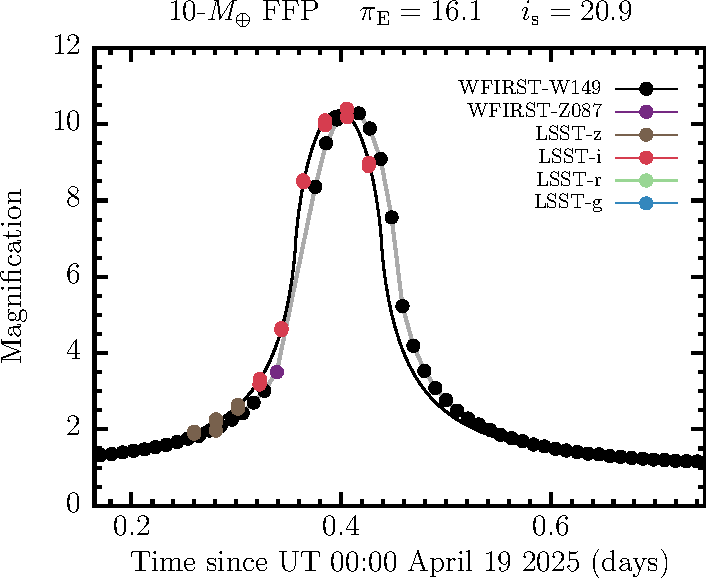
\includegraphics[width=0.5\linewidth]{figs/WFIRST/lsst_lsstm+10_0_7220351_320_det_lc.pdf}
\caption{The light curve of a $10 M_{\oplus}$ planet with a microlensing parallax
mass measurement from simultaneous WFIRST and LSST observations.
\label{fig-lc}}
\end{figure}

WFIRST planetary microlensing events will greatly improve our
understanding of not only rogue planets population but also cold giants similar to
Uranus or Neptune and smaller mass planets on wide orbits. Cold giants
cannot be studied using techniques other than microlensing and
WFIRST gives us a unique opportunity to detect a statistically significant
number of wide orbit planets. Even though the wide orbit planets will be detected,
their properties may not be well constrained by WFIRST or it may be hard to distinguish
between a wide orbit planet and a rogue planet, particularly for planets on the widest
orbits or when the source trajectory does not closely approach the host star.
The two main parameters that can be derived for bound planets are
the mass ration, $q$, and the projected separation ,$s$, in units of Einstein radius.
Wide orbit planet adds an additional peak to the otherwise
standard microlensing light curve produced by the planet host.
The time separation of the two peaks, $\Delta t$, is directly related
to the planet projected separation:
\begin{equation}
 \Delta t =  t_{\rm E}(s - {1/s}) \ .
\end{equation}
Typical value of $t_{\rm E}$ is $25~{\rm days}$, hence, for a wide
separation planet ($s$ on the order of a few) $\Delta t$ will be
comparable to the length of a single WFIRST session i.e., $72~{\rm days}$.
Even though WFIRST will be able to observe the planetary anomaly,
it may not observe the host event and hence poorly constrain planet properties. Deep low-cadence LSST
monitoring of the WFIRST microlensing field over whole bulge observing season
will reveal the peaks of planet host microlensing events that are unobservable
to the WFIRST and will help to constrain projected separation and mass ratio.


% --------------------------------------------------------------------

\subsection{A Proposed Observing Strategy}
\label{sec:\secname:proposal}

Based on the desiderata above, we
propose simultaneous high cadence observations of the WFIRST microlensing fields
by LSST during each
of the six 72-day WFIRST exoplanet microlensing survey sessions. These
will allow microlensing parallax measurements to determine the distances
and masses of a representative sub-sample of the rogue planets found by
the WFIRST microlensing survey. These measurements will be crucial for
the interpretation of WFIRST's rogue planet discoveries, and they
cannot be obtained by another method.

We also propose continuous monitoring of the WFIRST microlensing fields
at a cadence of one observation per day
starting a year before and ending a year after the WFIRST microlensing survey.
This will allow us to constrain the presence of a host star for rogue planet candidates and,
if the host is detected, measure the planet-host mass ratio and projected separation.

A single LSST pointing, centered on the WFIRST microlensing
fields, would cover all 10 WFIRST microlensing fields.

For our preliminary estimates of the high-cadence observing, we assume
that the bulge is observed every 30 minutes when the bulge is at
an airmass of $< 2.5$ for 76-day observing runs (each 72-day WFIRST observing
season plus 2 days on either side). Each visit consists of 3 exposures,
one 2 sec exposure followed by two 15 sec exposures. With a 2 sec readout
and 1 sec for the shutter to open and close, this comes to 39 sec on target
per visit (since the final readout can be done while slewing).
If we assume a 30 deg slew in Azimuth before and after each microlensing pointing, the slews
to and from the target should take 22 sec, which is 12 sec above the average. So,
each visit will take 61 sec out of the regular observing sequence.
The number of observations per night, assuming a 30 minute cadence, for
a Spring 2025 observing session are given in \autoref{tab:wfirst_ml_survey}. We will require
that these observations be taken in the $riz$ or $y$ filters with at
least 3 (or 0) observations in each filter per night. The total number
of observations with this observing plan is 649 or 11.0 hour per
76-day observing session or 3894 observations and 66.0 hours for
all the high cadence observations that we propose.

\begin{table}
\begin{tabular}{ c c }
{\bf days} & {\bf Observations} \\
\hline
Feb 10-16     &  3 \\
Feb 17-23     &  4 \\
Feb 24-Mar 1  &  5 \\
Mar 2-8       &  6 \\
Mar 9-14      &  7 \\
Mar 15-21     &  8 \\
Mar 22-28     &  9 \\
Mar 29-Apr 4  & 10 \\
Apr 5-10      & 11 \\
Apr 11-17     & 12 \\
Apr 18-24     & 13 \\
Apr 25-28     & 14 \\
\end{tabular}
\caption{Observations per night at 30 minute cadence for a Spring
WFIRST microlensing survey.}
\label{tab:wfirst_ml_survey}
\end{table}

These observing plans can be altered by changing the cadence of the high
cadence observations from once every 30 minutes to once every 15, 60,
or 120 minutes, or we could change the number of WFIRST microlensing
observing seasons that were covered. We have not yet simulated the
different observing cadences, however.

The low-cadence (1 observation per day) observations taken when WFIRST
is not observing, would consist of 1270 visits if we assume that
the observations are not taken during the time when the $u$ filter is
on the telescope (this is assumed to be 1/6 of the time). The low-cadence
off-season observations then total 21.5 hours. Low- and high-cadence
observations will take a total of 87.5 hours over 8 years.



% --------------------------------------------------------------------

\subsection{Metrics}
\label{sec:\secname:metrics}

\subsubsection{High-cadence observations}

\autoref{tab:wfirst_ml_results}
shows the results of our simulations of the combined proposed WFIRST-LSST
observing program. We assume that there is 1 planet per main sequence
star at each of $1\,M_\oplus$, $10\,M_\oplus$, and $100\,M_\oplus$.
This is the 1-$\sigma$ lower limit found by \citet{2011Natur.473..349S} at
$M_{\rm L} \approx 300\,M_\oplus$, and the rogue planet mass function is
thought to increase toward lower masses, so this is a conservative
assumption. The first row gives the number of events that will be
observed by WFIRST. The second row gives the number of these events
with source SDSS-$i \leq 23$, which were the only events included in the
LSST simulations. The third and fourth rows give the number of these events
with LSST-WFIRST microlensing parallax measurements and the number
with full mass measurements. It is this row that indicates the
value of the LSST observations.

\begin{table}
\begin{tabular}{lcccc}
Category & $100\,M_\oplus$ & $10\,M_\oplus$ & $1\,M_\oplus$ & Total \\
\hline
WFIRST-events    &   417   &         127    &         33    &  577  \\
$i \leq 23$      &    88   &          30    &         13    &  131  \\
$\pi_{\rm E}$ measured &    22   &           8.2  &          2.7  &   32.9 \\
$M_{\rm L}$ measured   &    5.9  &           3.4  &          1.5  &   10.8 \\
\end{tabular}
\caption{Number of rogue planets of the given mass detected, assuming
one such planet per main sequence star, and our proposed LSST observation
program.}
\label{tab:wfirst_ml_results}
\end{table}

One can see from the final column that the LSST observations should
yield more than 30 rogue planet microlensing parallax measurements and
more than 10 rogue planet mass measurements.
%
These are measurements that cannot be made by other methods, as there is
currently no other known way to measure the mass distribution and abundance
of dark, isolated objects.
% \textbf{THE PREVIOUS SENTENCE NEEDS MORE JUSTIFICATION.}
%
In addition, this program would
also yield masses for a somewhat larger number of bound planets
\citep{2003ApJ...591L..53G}, although many of these will have their
masses determined by other means as well.

For a proxy for a Figure of Merit, we select the product of the numbers of
rogue planet microlensing parallax measurements $\pi_{\rm E}$
and rogue planet mass measurements $M_{\rm L}$.
% Added by PJM:
We expect this quantity to be simply related to the ultimate precision
on any rogue planet population hyperparameter we may try to infer from
the LSST-WFIRST sample.
Some additional
work is still needed to test and develop this metric so that it can be easily incorporated into the MAF based on OpSim runs.
The value of this product is 355 for our straw man program.


\subsubsection{Low-cadence observations}

LSST observations will improve models for WFIRST planetary events
in a number of ways but here we focus on detection of the planet
host peak if it was missed and poorly constrained by WFIRST. We simulate
a population of planets with masses of $0.1\,M_\oplus$, $1\,M_\oplus$,
and $10\,M_\oplus$ that follow logarithmic mass function with
normalization extrapolated from Cassan et al. (2012). We narrow the sample of
planets detected by WFIRST in a number of steps. First, we reject the events
with host peak during the LSST high-cadence observations, i.e., during one of six
76-day long campaigns. Second, we exclude the events with host event reaching
at least $0.75$ of the event maximum flux increase, because in these cases WFIRST
data will strongly constrain the host peak even though it is not fully observed.
Third, we require at least a single LSST observation within $\pm0.05t_{\rm E}$ of
the host peak and the magnified source flux to be brighter than SDSS-$z$ of $23~{\rm mag}$.
The expected number of $0.1\,M_\oplus$, $1\,M_\oplus$, and $10\,M_\oplus$
planets for which host peak is detected are 2.1, 8.7, and 36.9, respectively.
We chose a sum of those as a proxy for a Figure of Merit. For the observing strategy
presented above the value of this FoM is 47.7. If a maximum airmass is chosen to be
2.0 instead of 2.5, then the requested time decreases by $6\%$ and FoM decreases by $12\%$.
The metric is based solely on the distribution of peak times and source magnitudes
for a given WFIRST simulation, so once this is set, the metric can
be easily computed for any OpSim run.


% Quantifying the response via MAF metrics: definition of the metrics,
% and any derived overall figure of merit.

% % --------------------------------------------------------------------
%
% \subsection{OpSim Analysis}
% \label{sec:\secname:analysis}
%
% OpSim analysis: how good would the default observing strategy be, at
% the time of writing for this science project?
%
%
% % -------------------------------------------------------------------- % %

\subsection{Discussion}
\label{sec:\secname:discussion}

The rough estimates of our metrics and Figure of Merit given above were
carried out using a very simple model for the LSST observations we
have proposed. We would hope to refine this analysis using the output
of an `OpSim` run where the WFIRST+LSST microlensing program was included
as an additional special survey, and our Figure of Merit coded in the
MAF. We do not expect the impact of this special survey on other science cases
to be high, as it would only need 12 hours per year in total. The risk
seems similar, but smaller than that of a Deep Drilling Field.

Other science teams may find it useful to think of the WFIRST+LSST microlensing
survey as a medium deep drilling field located in the bulge: it would be interesting
to see how some of the Milky Way, galactic transient, and  stellar variable
metrics changed with the addition of this proposed survey.


% ====================================================================

\subsection{Conclusions}

Here we answer the ten questions posed in
\autoref{sec:intro:evaluation:caseConclusions}:

% Answered by DB 08/09/16,
% minor changes by RP 08/10/16, added by MP 08/15/16

\begin{description}

\item[Q1:] {\it Does the science case place any constraints on the
tradeoff between the sky coverage and coadded depth?}

\item[A1:] No: this is irrelevant to the microlensing survey. We have
specific cadence requirements and much less interest in coadded depth.

\item[Q2:] {\it Does the science case place any constraints on the
tradeoff between uniformity of sampling and frequency of sampling?}

\item[A2:] During the microlensing survey, we must maintain the
requested 30 or 15 minute cadence to within 3 minutes. Outside of the
microlensing survey, we must maintain our daily cadence to within 4
hours.

\item[Q3:] {\it Does the science case place any constraints on the
tradeoff between the single-visit depth and the number of visits
(especially in the $u$-band where longer exposures would minimize the
impact of the readout noise)?}

\item[A3:] There is no trade-off: we cannot reduce our cadence.

\item[Q4:] {\it Does the science case place any constraints on the
Galactic plane coverage (spatial coverage, temporal sampling, visits per
band)?}

\item[A4:] All of the observations must take place in a field that we
will specify near the Galactic Center, at Galactic coordinates of
roughly $l = 1$~deg, $b = -1.5$~deg.

\item[Q5:] {\it Does the science case place any constraints on the
fraction of observing time allocated to each band?}

\item[A5:] We  require observations to be in a passband at least as red
as the $r$-band, i.e. that 0\% of the observing time be in the $u$ or
$g$-bands.

\item[Q6:] {\it Does the science case place any constraints on the
cadence for deep drilling fields?}

\item[A6:] Our proposal may amount to a new deep drilling field in the
central Galactic bulge. In this case, the constraints would be 15 or 30
min cadence during 6 WFIRST microlensing seasons, and 1 day cadence
otherwise.

\item[Q7:] {\it Assuming two visits per night, would the science case
benefit if they are obtained in the same band or not?}

\item[A7:] We propose between 3 and 14 visits per night during the
WFIRST microlensing survey, and 1 visit per night otherwise. We have no
restrictions other than the restriction to no visits in the $u$ and
$g$-bands.

\item[Q8:] {\it Will the case science benefit from a special cadence
prescription during commissioning or early in the survey, such as:
acquiring a full 10-year count of visits for a small area (either in all
the bands or in a  selected set); a greatly enhanced cadence for a small
area?}

\item[A8:] We require many visits during the WFIRST exoplanet
microlensing seasons, starting in 2025. Before that, we require only one
observation per night.

\item[Q9:] {\it Does the science case place any constraints on the
sampling of observing conditions (e.g., seeing, dark sky, airmass),
possibly as a function of band, etc.?}

\item[A9:] There is value in relaxing a default airmass constraint,
where it would mean no observations were taken. We only have strict
cadence requirements.

\item[Q10:] {\it Does the case have science drivers that would require
real-time exposure time optimization to obtain nearly constant
single-visit limiting depth?}

\item[A10:] No.

\end{description}


% ====================================================================

\navigationbar
